\chapter{雜類話題I}
\section{2016年1月11日 (Instructor: Vivian)}
\subsection{幼兒教育}
\subsubsection*{需要掌握的單詞短語}
\begin{multicols}{2}
\begin{itemize}
  \itemsep0em
  \item Childcare: 托兒所
  \item Preschool: 幼兒園
  \item \hilight{Kindergarten\footnote{在澳洲, kindergarten請勿翻譯成幼兒園!} - 學前班}
  \item day care: 日托
  \item 遊戲小組: play group
  \item \hilight{全日制非全日制}: Fill-time 和 Part-time\footnote{這裡不要翻譯成全職兼職}
  \item \textbf{AMEP}: Adult Migrant English Program (成人移民英語課程)
  \item benefit: 福利金
  \item 接種記錄 - Immunisation / Vaccination record.
\end{itemize}
\end{multicols}

\subsubsection*{需要掌握的句型}
\begin{itemize}
  \itemsep0em
  \item 想要瞭解更多信息: get more information about ... 或 to enquire about ...
  \item 它們分別提供***: do they \hilight{each} provide ... ?
  \item 有資格: be eligible \hilight{for} sth.
  \item 剛好知道: happen to know (我刚好在学法语: I happened to be learning French.)
\end{itemize}

\subsection{抑鬱症}
\mybox{\centering \textbf{注意}: 本對話的更多筆記被歸納到專題里的``宣傳冊和傳單", 請參考目錄進行查找!}
\subsubsection*{需要掌握的單詞短語}
\begin{itemize}
  \itemsep0em
  \item 抑鬱 / 焦慮: depression / anxiety
  \item 喜歡獨處: enjoy \hilight{solitude ($n.$)}
\end{itemize}

\subsubsection*{需要掌握的句型}
\begin{itemize}
  \itemsep0em
  \item 老實說: to be honest / honestly speaking.
  \item 如釋重負: I feel much relieved.
  \item 阻止某人: stop sb. from ...
  \item 照顧好某人: take good care of sb. / look after sb. very well.
  \item 建議做某事: suggested (that) sb. (should) do sth. (不要用成to do!)
\end{itemize}

\subsection{授權書}
\subsubsection*{需要掌握的單詞短語}
\begin{multicols}{2}
\begin{itemize}
  \itemsep0em
  \item 關於授權委託的一系列表達:
  \begin{enumerate}
  \itemsep0em
    \item 授權書: \hilight{Power of Attorney}
    \item 授權人 / 委託人: principal
    \item 代理人: attorney
    \item 公共信託人: public trustee
    \item 提名: nominate
  \end{enumerate}
  \item (老年)痴呆: \hilight{(senile) dementia}, 突發的: \hilight{onset}
  \item 靜脈曲張: varicose veins\footnote{靜脈曲張是指由於血液淤滯、靜脈管壁薄弱等因素,導致的靜脈迂曲、擴張。身體多個部位的靜脈均可發生曲張,比如\\痔瘡其實就是一種靜脈曲張,臨床可見的還有食管胃底靜脈曲張、精索靜脈曲張及腹壁靜脈曲張等等。}
  \item \hilight{轉介信}: referral letter
  \item 遺傳性的: hereditary, 抗生素: anti-biotics.
  \item 副作用: side effect, 後遺症: after effect.
  \item 藥物: medication, 抗藥性: drug resistance.
  \item 控制(病情發展): manage = control
\end{itemize}
\end{multicols}

\subsubsection*{需要掌握的句型}
\begin{itemize}
  \itemsep0em
  \item 代表某人: act on one's behalf.
  \item 使某人享有某權利: entitle $sb.$ to do ...
  \item 痛得睡不著覺: I can't fall asleep due to the pain.
\end{itemize}

\section{2016年1月12日 (Instructor: Chris)}
\subsection{買車}
\subsubsection*{需要掌握的單詞短語}
\begin{multicols}{2}
\begin{itemize}
  \itemsep0em
  \item (車)品牌: make ($n$)
  \item 吸引人: attractive / \hilight{appealing}
  \item 一團火焰: flame
  \item 方向盤: steering wheel
  \item 變速: gear / transmission
  \item 變速種類: manual / auto / semi-auto
  \item 選色卡: colour chart
  \item 金屬灰: Metallic grey
\end{itemize}
\end{multicols}

\subsubsection*{需要掌握的句型}
\begin{multicols}{2}
\begin{itemize}
  \itemsep0em
  \item 考慮好: made up my mind.
  \item (事情)是這樣的: here is the thing / well ...
  \item 傾向於: It tends to be ... \hilight{(一定要加s)}
  \item 大約在某時: \hilight{or so} = around = duration / time
  \item 關於付款和錢的一些表達:
  \begin{enumerate}
  \itemsep0em
    \item \textbf{信用卡分期付款}: pay by credit \hilight{in instalments}.
    \item \textbf{一次性付清}: in lump sum.
    \item \textbf{首付}: down payment.
    \item \textbf{手頭有點緊}: I'm short on cash.
    \item \textbf{估價}: value / valuation.
    \item \textbf{升降值}: appreciation / depreciation.
  \end{enumerate}
\end{itemize}
\end{multicols}

\subsection{入室盜竊}
\subsubsection*{需要掌握的單詞短語}
\begin{multicols}{3}
\begin{itemize}
  \itemsep0em
  \item 入室盜竊: burglary / burgle
  \item 盜賊: burglar
  \item 萬能鑰匙: bump key
  \item 防萬能鑰匙的鎖: anti-bump locks
  \item 旅行支票: \hilight{traveller's} check
  \item 大使館: embassy
  \item 領事館: consulate
  \item 心安: peace of mind
\end{itemize}
\end{multicols}

\subsubsection*{需要掌握的句型}
\begin{multicols}{3}
\begin{itemize}
  \itemsep0em
  \item \hilight{永遠: for good} = forever
  \item 上了保險: be insured
  \item 企圖做但未遂: attempt
\end{itemize}
\end{multicols}

\subsection{家長老師見面}
\mybox{\centering \textbf{注意}: 本對話的更多筆記被歸納到專題里的關於``和學校有關的詞", 請參考目錄進行查找!}
\subsubsection*{需要掌握的單詞短語}
\begin{multicols}{2}
\begin{itemize}
  \itemsep0em
  \item 闖禍 / 惹麻煩: act up
  \item 想出: figure out / come up with / work out
  \item 謙遜的: humble
  \item 家長會: parent-teacher interview
\end{itemize}
\end{multicols}

\subsubsection*{需要掌握的句型}
\begin{multicols}{2}
\begin{itemize}
  \itemsep0em
  \item 過獎了: I'm flattered
  \item 放心了: be relieved.
\end{itemize}
\end{multicols}

\subsection{車禍}
\subsubsection*{需要掌握的單詞短語}
\begin{multicols}{3}
\begin{itemize}
  \itemsep0em
  \item 租賃中介: rental agency
  \item 周到: thoughtful
  \item 擋風玻璃: windshield
  \item 護欄: guardrail
  \item 救助人員: \hilight{paramedics}
\end{itemize}
\end{multicols}

\subsubsection*{需要掌握的句型}
\begin{itemize}
  \itemsep0em
  \item 嚇壞了: be freaked out
  \item 撞到了某處: \hilight{sb. + body part + on / against + place.}
  \item 受傷很重 / 很輕: sb. + be + \hilight{severely / mildly} injured.
  \item 腹部劇痛: sharp pain \hilight{in the} abdomen.
  \item 翻車: went up side down / flipped over.
  \begin{center}
    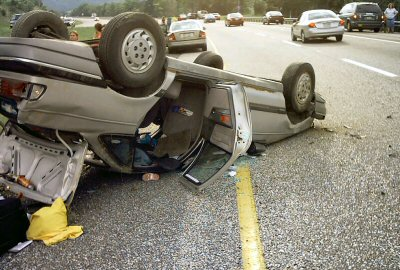
\includegraphics[scale=1.8]{pics/flip-over}
  \end{center}
  \item (車子)撞到了某處: \hilight{crash / bump / collide / run into ...}
\end{itemize}

\vspace{15mm}

\begin{center}
  \textbf{************ END OF THE DAY ************}
\end{center}

\newpage

\section{2016年1月18日 (Instructor: Vivian)}
\subsection{結核病}
\mybox{\centering \textbf{注意}: 本對話的更多筆記被歸納到專題里的關於``和疾病有關的詞", 請參考目錄進行查找!}
\subsubsection*{需要掌握的單詞短語}
\begin{multicols}{2}
\begin{itemize}
  \itemsep0em
  \item file: 資料, 病例\footnote{file這個詞在醫院有關的對話中不要翻譯成``檔案"!}
  \item 異常: abnormal ($adj.$) / abnormality ($n.$)
  \item 定期健康檢查: regular health checks
  \item 經常鍛鍊: regular exercise \hilight{(不要翻譯成定期鍛鍊)}
  \item 年齡的增長: \hilight{aging}, 可治癒的: \hilight{curable}
  \item 痰中帶血: blood \hilight{stained} sputum
  \item 盜汗: night sweating
  \item 慢性的 / 急性的: chronic / acute
  \item 驟然: in a short period
  \item 餐具: crockery
  \item 家用物品: Household items
\end{itemize}
\end{multicols}

\subsubsection*{需要掌握的句型}
\begin{itemize}
  \itemsep0em
  \item 沒什麼(特別的)問題: Nothing in particular.
  \item 我三周前開始咳嗽: I \hilight{have been coughing} since 3 weeks ago.
  \item 我體重突然下降: I have sudden weight loss.
  \item 這對嗎? \hilight{It is so?} / Is it right?
\end{itemize}

\subsubsection*{特別注意}
\begin{itemize}
  \itemsep0em
  \item 這篇文章出現了 sth. \hilight{and/or} sth. 翻譯時不要漏了其中一種情況. 
\end{itemize}

\subsection{醫療事故}
\subsubsection*{需要掌握的單詞短語}
\begin{multicols}{2}
\begin{itemize}
  \itemsep0em
  \item 手術器械: surgical utensil
  \item 醫療事故: medical incident
  \item 訴訟: lawsuit / litigation
  \item 提交(訴訟): lodge
  \item 當值律師: duty solicitor
  \item 法律程序: legal procedure
  \item 例行檢查: regular check-up
  \item 意向: preference (這裡不要翻譯成偏好)
  \item 照價賠償: pay agreed amount.
\end{itemize}
\end{multicols}

\subsubsection*{需要掌握的句型}
\begin{itemize}
  \itemsep0em
  \item 為這件事故感到沮喪: upset \hilight{over} this incident.
  \item 一大筆錢: large sum of money.
  \item 庭外和解: out of court settlement 或 settle the case / matter out of court.
  \item 幫助我庭外索賠: Help me with the claim / get the compensation outside the court.
\end{itemize}

\subsection{新移民}
\subsubsection*{需要掌握的單詞短語}
\begin{itemize}
  \itemsep0em
  \item 住址: \hilight{residential} address
  \item 好時機: good timing
  \item 優惠: concession
  \item 配偶移民: partner migration (scheme)
  \item TAFE (Technical and Further Education) 技術與繼續教育學院, 也可以不翻譯
\end{itemize}

\subsubsection*{需要掌握的句型}
\begin{itemize}
  \itemsep0em
  \item 我沒有別的選擇, 只能... : I don't have any other options, but to ...
\end{itemize}

\subsection{老年痴呆}
\subsubsection*{需要掌握的單詞短語}
\begin{multicols}{2}
\begin{itemize}
  \itemsep0em
  \item 婆婆: mother-in-law
  \item 阿茲海默症: Alzheimer's disease\footnote{阿茲海默症侵襲人的腦部;它並非正常的老化現象。得到阿茲海默症的人會漸漸的喪失記憶並且出現語言和情緒上的\\障礙。}
  \item 失憶症: amnesia
  \item 大小便失禁: incontinent
  \item (身體的)官能: faculty
  \item 幻覺: \hilight{hallucinations / delusion}
  \item 不安: restless
\end{itemize}
\end{multicols}

\subsubsection*{需要掌握的句型}
\begin{multicols}{2}
\begin{itemize}
  \itemsep0em
  \item 得了***病: has got ... = developed ...
  \item 不止這些: that's not all
  \item 尿床: wet someone's bed
  \item 坐不住: can't sit still
  \item 搓拉皮膚: rub and pull skin
  \item 怎麼可能: How could this be possible?
  \item 50多歲: in 50's.
  \item 身體壯得像頭牛: As tough as \hilight{nails}\footnote{不要直接把``牛"翻譯出來!}
  \item 並不常見: It is \hilight{not uncommon}.
\end{itemize}
\end{multicols}

\subsection{兒童發展}
\subsubsection*{需要掌握的單詞短語}
\begin{multicols}{2}
\begin{itemize}
  \itemsep0em
  \item 素質: potential
  \item 滿意: happy with\footnote{satisfy一般指比較大的生理或心理的滿足}
  \item 努力去做: struggle to do
  \item 阻礙以後發展: hold sb. back
  \item 一同參與: getting involved
  \item 健康障礙: physical barriers
\end{itemize}
\end{multicols}

\subsubsection*{需要掌握的句型}
\begin{itemize}
  \itemsep0em
  \item 他在學校表現如何: How is his performance at school?
  \item 在某人的這個年齡: someone of his / her age.
\end{itemize}

\vspace{15mm}

\begin{center}
  \textbf{************ END OF THE DAY ************}
\end{center}

\newpage

\section{2016年1月19日 (Instructor: Chris)}
\subsection{度假旅行}
\mybox{\centering \textbf{注意}: 本對話的更多筆記被歸納到專題里的關於``和暈車暈船有關的症狀", 請參考目錄進行查找!}
\subsubsection*{需要掌握的單詞短語}
\begin{multicols}{2}
\begin{itemize}
  \itemsep0em
  \item 旺季: peak season
  \item 淡季: off-peak season
  \item 平季: \hilight{shoulder} season
  \item 爬行動物: reptile
  \item 觀鯨旅遊: whale watching
  \begin{center}
    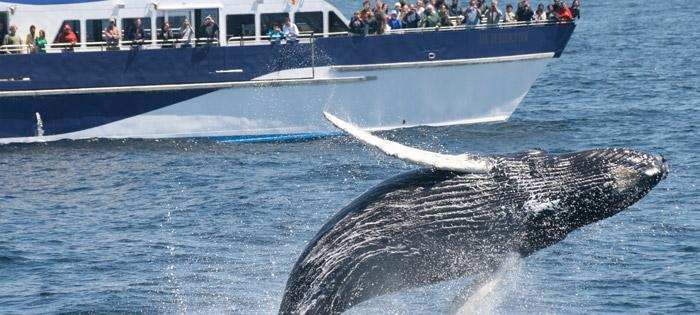
\includegraphics[scale=.3]{pics/whale-watching}
  \end{center}
  \item 假日套餐: holiday \hilight{packages}
  \item 度假村: resort
  \item 近距離的: up close
  \item 日光浴: sunbathing
  \item 暈動症: motion sickness
  \item 甲板: deck
  \item 海上巡航: cruise
  \item 帶氧氣瓶潛水: Scuba diving
  \item 浮潛: Snorkelling
  \item (旅遊)團: tour (不要翻譯成group)
  \item \hilight{舒活筋骨: stretch up}
  \item 臨時預定: \hilight{tentative} booking
  \item 鞋架: shoe rack
\end{itemize}
\end{multicols}

\subsubsection*{需要掌握的句型}
\begin{itemize}
  \itemsep0em
  \item 靠海別墅: villa on the beach
  \item 也有道理: fair enough
  \item 措施機會(非意外): miss out on ...
\end{itemize}

\subsection{新移民資訊 (Hurstville)}
\mybox{\centering \textbf{注意}: 更多筆記被歸納到專題里的``和銀行有關的詞"和``宣傳冊和傳單", 請參考目錄查找!}
\subsubsection*{需要掌握的單詞短語}
\begin{itemize}
  \itemsep0em
  \item 公證件: \hilight{notarised} version (不是certified)
  \item Hurstville可以不翻譯!
\end{itemize}

\subsubsection*{需要掌握的句型}
\begin{itemize}
  \itemsep0em
  \item 本應該做但沒做: should have done ...
\end{itemize}

\subsection{支氣管炎}
\subsubsection*{需要掌握的單詞短語}
\begin{multicols}{2}
\begin{itemize}
  \itemsep0em
  \item 口水: saliva
  \item (吐)痰: \hilight{(bring up)} sputum / phlegm
  \item 上氣不接下氣/氣短: short of breath
  \item 併發症: complications
  \item 甲狀腺:thyroid gland
  \item 碘: iodine
  \begin{center}
    \includegraphics[scale=.7]{pics/iodine}
  \end{center}
  \item 肺炎: pneumonia
  \item 青霉素: penicillin
  \begin{center}
    
\includegraphics[scale=.2]{pics/penicillin}
  \end{center}
  \item 乳製品: dairy products
  \item 花粉: pollen
  \item 粉塵: dust
  \item 撲熱息痛: paracetamol
  \item 抗組胺藥: antihistamine
  \item 安眠藥: sleeping pills
  \item 止疼藥: analgesic ($adj$ \& $noun$) / painkiller
  \item 粘稠的痰: \hilight{thick} sputum
  \item 黃綠色: \hilight{greenish yellow}\footnote{其他顏色可以用類似方法表法, 注意調換順序}
\end{itemize}
\end{multicols}

\subsubsection*{需要掌握的句型}
\begin{itemize}
  \itemsep0em
  \item 對...過敏: be allergic to...
  \item 以防萬一: for precaution / to be on the safe side
  \item 那時才發現: found back then
  \item 這可能是其中的原因嗎? Could it be the reason?
  \item 整個療程: full \hilight{course} of ...
  \item 高壓150, 低壓90: The blood pressure is 150 \hilight{over} 90.
\end{itemize}

\subsection{泌尿疾病}
\mybox{\centering \textbf{注意}: 本對話的更多筆記被歸納到專題里的關於``不同的疼法", 請參考目錄進行查找!}
\subsubsection*{需要掌握的單詞短語}
\begin{itemize}
  \itemsep0em
  \item 核磁共振: MRI (Magnetic Resonance Imaging)
  \item 尿道: Urinary tract
  \item 性病: Sexually Transmitted Diseases / Venereal Diseases
  \item 灼燒感: burning sensation
  \item 前列腺腫大: \hilight{enlarged} prostate
  \item (思想)開放: open / open-minded
  \item \hilight{空腹: fast}
  \item 頭巨痛: splitting headache
\end{itemize}

\subsubsection*{需要掌握的句型}
\begin{multicols}{2}
\begin{itemize}
  \itemsep0em
  \item 我每次排尿的時候都會感覺疼:
  \begin{enumerate}
    \itemsep0em
    \item It hurts everytime I pass water.
    \item It is painful everytime I pass urine. 
    \item I have pain everytime I pass water.
  \end{enumerate}
  \item 無意冒犯: no offence = with respect
  \item 你沒有冒犯到我: Not taken.
  \item 我不能忍受: I can't bear / take / stand / put up with ...
\end{itemize}
\end{multicols}

\subsection{骨折(三級)}
\mybox{\centering \textbf{注意}: 本對話的更多筆記被歸納到專題里的關於``不同的麻醉方式", 請參考目錄進行查找!}
\subsubsection*{需要掌握的單詞短語}
\begin{multicols}{2}
\begin{itemize}
  \itemsep0em
  \item 內部固定: Internal fixation
  \item 外部夾板: External splint
  \item 石膏拖: plaster cast
  \item \hilight{瘸著走路: walk with a limp}
  \item 合適的急救: proper first aid.
  \item 大/小腿骨: thigh / calf bone
  \item 產假: maternity leave
  \item 事假: personal leave
  \item 喪假: funeral leave
  \item 長期服務假: long service leave
\end{itemize}
\end{multicols}

\vspace{15mm}

\begin{center}
  \textbf{************ END OF THE DAY ************}
\end{center}
\newpage

\section{2016年1月25日 (Instructor: Vivian)}
\subsection{就業幫助}
\subsubsection*{需要掌握的單詞短語}
\begin{itemize}
  \itemsep0em
  \item 非政府機構: Non-Government Organisation (NGO), 津貼: benefit / allowance
  \item 機械學: Machics, 機電維修: Mechanical \hilight{maintenance}, 機床廠: Machine tools / parts factory
  \item 偏僻的: isolated / remote
  \item 重拾自信: regain self-esteem, 自食其力: support themselves
  \item 個人\hilight{信息}: Personal \hilight{detail} (detail這裡不用翻譯成細節)
  \item 固定的 / 穩定的工作: Permanent employment (不要翻譯成永久的)
  \item (學歷)被承認: recognised
  \item 自卑: self-abased / self-inferior / low self-esteem
  \item 自我感覺良好(貶義): high self-esteem
\end{itemize}

\subsubsection*{需要掌握的句型}
\begin{itemize}
  \itemsep0em
  \item 我是(汽車)維修工: I'm a/an (auto) mechanic.
  \item 我想不明白...: I wonder why...
  \item 你讓我怎麼辦?:
  \begin{enumerate}
    \itemsep0em
    \item What else can I do?
    \item What do you expect me to do?
    \item What am I suppose to do?
  \end{enumerate}
  \item \hilight{省省吧, 不要說廢話: Just save it!}
  \item 配合某人走過場: Cooperate with sb. to \hilight{go through the formalities}.
  \item 在中國獲得的學歷: qualification obtained / acquired in China.
\end{itemize}

\subsubsection*{其他}
\begin{itemize}
  \itemsep0em
  \item ``學歷"翻譯成qualification, 學歷從低到高分別是 certificate, diploma和degree, 其中degree代表至少大學的學歷.
\end{itemize}

\subsection{種族歧視}
\subsubsection*{需要掌握的單詞短語}
\begin{itemize}
  \itemsep0em
  \item \hilight{背地裡: behind someone's back} (without a person's knowledge and in an unfair way.)
  \item 小舅子: brother-in-law
  \item 英文書: books in English
  \item 店主 / 店員: shop keeper / shop assistant, 白人: caucasian
  \item 出去: go out (走出去) / get out (滾出去, 用於罵人)
  \item 在場: at the scene
\end{itemize}

\subsubsection*{需要掌握的句型}
\begin{itemize}
  \itemsep0em
  \item 我收到了 / 遭受了歧視:
  \begin{enumerate}
    \itemsep0em
    \item I suffered discrimination.
    \item I was discriminated against...
    \item I was subjected to / a subject of discrimination.
  \end{enumerate}
  \item 拒絕為我服務: refuse to serve me
  \item 被視為: can be considered / regarded as
  \item 聽見有人背後說: I heard a voice behind.
  \item 聽了以後很不爽: I felt very uncomfortable after heard that.
  \item 回嘴:
  \begin{enumerate}
    \itemsep0em
    \item respond with a comeback.
    \item answer sb. back.
  \end{enumerate}
  \item 你怎麼認為的?: How did you take that?
  \item 依照種族背景: refer to ethnic background
  \item 目睹這個事情: Witness ($noun.$ + $verb.$, 這裡是動詞) the incident.
  \item 這是 / 那是我第一次做某事:
  \begin{enumerate}
    \itemsep0em
    \item This is my first time of doing something.
    \item That was the first time that I have done something.
  \end{enumerate}
\end{itemize}

\subsubsection*{其他}
\begin{itemize}
  \itemsep0em
  \item 歧視(discrimination) 一般有關於 gender / sexual, age 和 radial的
\end{itemize}

\subsection{人生低谷}
\subsubsection*{需要掌握的單詞短語}
\begin{itemize}
  \itemsep0em
  \item 搞砸: screwed up / mess up
  \item 苟延殘喘: keep struggle
  \item 自我形象: self image
  \item \hilight{潦而不倒: down but not out}
  \item \hilight{窮困潦倒: down and out}, 關於本俚語的來源和解釋請點\href{http://www.ept-xp.com/?ID=2204020903}{這裡}
\end{itemize}

\subsubsection*{需要掌握的句型}
\begin{itemize}
  \itemsep0em
  \item 我甚至不能...: I can't even managed to...
  \item 在我20多歲: In my 20's.
  \item 錯誤地歸咎: sb. wrongly blame sb. for sth.
  \item 照鏡子:
  \begin{enumerate}
    \itemsep0em
    \item I look into the mirror.
    \item I look at myself in mirror.
  \end{enumerate}
  \item 我還有救嗎: Do I have any hope?
\end{itemize}

\subsubsection*{其他}
\begin{itemize}
  \itemsep0em
  \item Overwhelm (壓倒性的):
  \begin{enumerate}
    \itemsep0em
    \item 太讓人受不了了: something is overwhelming.
    \item 被制服的, 被壓倒, 勢不可擋的: be overwhelmed.
  \end{enumerate}
\end{itemize}

\subsection{丟失包裹}
\mybox{\centering \textbf{注意}: 本對話的更多筆記被歸納到專題里的關於``正確表示地點" 和話外音里的``悉尼地名奇葩翻譯".}
\subsubsection*{需要掌握的單詞短語}
\begin{itemize}
  \itemsep0em
  \item 平郵 (陸地或海運輸) / 普通郵件: surface mail
\end{itemize}

\subsubsection*{需要掌握的句型}
\begin{itemize}
  \itemsep0em
  \item 我上海的一個親戚給我發了包裹: A relative of mine in Shanghai sent me a parcel.
  \item 不可能...: There is no way...
  \item 與我\hilight{短住}: \hilight{stay} at my place.
  \item 不可能把地址弄錯: There is no way he could have gotten the address wrong.
\end{itemize}

\subsection{社工訪談}
\mybox{\centering \textbf{注意}: 本對話的更多筆記被歸納到專題里的關於``不同的救助補貼", 請參考目錄進行查找!}
\subsubsection*{需要掌握的單詞短語}
\begin{itemize}
  \itemsep0em
  \item 社工訪談: Social worker interview
  \item 電焊的活 / 焊工: welding job / welder
  \item elaborate = explain in detail
  \item 經濟不景氣: economic depression / recession / downturn
  \item 天主教學校: Catholic (C大寫) school
  \item 房租補貼: rent \hilight{assistant}
  \item 輔助性的家庭津貼: supplementary family allowance
\end{itemize}

\subsubsection*{需要掌握的句型}
\begin{itemize}
  \itemsep0em
  \item 經濟拮據: experiencing / having a financial difficulty.
  \item 鬱悶的是: \hilight{What's upsetting} is that...
  \item 經濟突然不景氣: economy went down suddenly / \hilight{in a sudden}.
  \item 我被炒了魷魚: I was laid off / dismissed / \hilight{made redundant}
  \item 我的問題一個接著一個: I have had problems one after another.
  \item 攢錢買: save money to buy...
  \item 不能收支平衡: can't make ends meet
  \item 很高興能幫你: I'm glad I have been able to help ... (用於回答Thank you for helping me.)
\end{itemize}

\subsection{非法修剪樹木}
\subsubsection*{需要掌握的單詞短語}
\begin{itemize}
  \itemsep0em
  \item 美甲, 修腳: manicure, pedicure (都是$v.$ + $n.$)
  \item 砍: chop, 樹幹: trunk, 樹枝: branch
  \item 同意: consensus = consent
  \item 出庭: appear in / at court.
  \item 當地政府: local \hilight{council}
  \item 批准: approval / permit ($verb.$ + $noun.$) / permission
  \item 專業技術人員: tradesperson = skilled person
  \item \hilight{技術培訓: trades training}
  \item (身心)健康: well-being
  \item 漏看: overlook
  \item 监督: oversee
\end{itemize}

\subsubsection*{需要掌握的句型}
\begin{itemize}
  \itemsep0em
  \item 莫名其妙: for no reason / without any reason.
  \item 因為某種原因: for some reasons.
  \item 有權力: be entitled to...
  \item 出庭: appear in / at court.
  \item 有一個關於你的訴訟: A lawsuit is being brought against you.
  \item 他收到一張傳票去\hilight{應訴} / 出庭作證: He has been served with a \hilight{subpoena} to \hilight{answer the charge in court} / \hilight{to give evidence in court}.
  \item 一張家庭暴力禁制令送達給某人(施暴的人): An apprehended domestic violence order has been \hilight{served} to sb.
  \item 又有什麼問題嗎??: What's wrong with that?? / Does it really matter?
  \item 反對: be opposed to / go against
  \item 英語說得比較好的朋友: Friend who speak \hilight{fairly} good English.
  \item 告某人:
  \begin{enumerate}
    \itemsep0em
    \item Sue $sb.$
    \item Take $sb.$ to court.
    \item Take legal action.
  \end{enumerate}
  \item 我的隔壁鄰居是個愛管閒事的人: My next-door neighbour is such a\hilight{nosy} person.
  \item 有權力: be entitled to...
\end{itemize}

\vspace{15mm}

\begin{center}
  \textbf{************ END OF THE DAY ************}
\end{center}

\newpage

\section{2016年1月28日 (Instructor: Chris)}
\subsection{毒品交易}
\mybox{\centering \textbf{注意}: 更多筆記被歸納到專題里的``和毒品有關的詞", 請參考目錄查找!}
\subsubsection*{需要掌握的單詞短語}
\begin{multicols}{2}
\begin{itemize}
  \itemsep0em
  \item 錄口供: make a statement
  \item 做筆錄: police interview
  \item \hilight{違法行為}: offense
  \item 酒保: bartender
  \begin{center}
    
\includegraphics[scale=0.3]{pics/bartender}
  \end{center}
  \item 挑釁: provoke ($v.$) / provocative ($adj.$)
  \item 攻擊性的, ``凶": aggressive
  \item 推責任: shift the blame / evade the responsibility\footnote{也可譯作``踢皮球"}
  \item 回憶, 記得: recollection $n.$
  \item 重新構思: reconstruction
  \item 黑手黨: Mafia
  \item 烈酒: spirit\footnote{注意和雪碧: Sprite 區分開!}
  \item 打火機, 火柴, : lighter / match
  \item 火把(火炬): torch
  \item 粗言穢語: abusive language
  \item 脾氣暴躁: grumpy
  \item 動手: start a fight / pick the fight\footnote{pick the fight不一定非是打, 也有可能是其他方式的衝突. 例句: I picked a fight \hilight{with} the guy beside me.}
  \item 同伴 (區別於friend): companions
  \item 搜身: frisk ($v.$)\footnote{例句: The passengers were frisked before they were allowed to board the plane. 俚語也可以譯作``扒竊".}
  \item 懸而未決的案子: cold case
\end{itemize}
\end{multicols}

\subsubsection*{需要掌握的句型}
\begin{itemize}
  \itemsep0em
  \item 我是被冤枉的: I'm innocent / \hilight{wronged}.
  \item 你一定要還我清白: You have to \hilight{clear my name}.
  \item 有人陷害我: I was set / framed by someone.
  \item 盡某人最大的能力: to the best of someone's ability
  \item 更別說: ... let alone / not to mention ... (不重要的放前面, 更重要的一些的放後面)\\例句: He is handsome and smart, not to mention being a good athlete.
  \item 趕走: take / escort\footnote{escort本身表示護送, 但依據上下文, 如果是被security guard護送, 則表示被趕走的意思.} someone out
  \item 例行公事: as a routine
  \item 有進展\hilight{第一時間}聯繫我: keep $sb.$ in the \hilight{loop} 或 keep $sb.$ updated / posted.
\end{itemize}

\subsection{尋求庇護者中心}
\subsubsection*{需要掌握的單詞短語}
\begin{multicols}{2}
\begin{itemize}
  \itemsep0em
  \item 尋求庇護者\footnote{尋求庇護者是指申請他國保護和居住權的人。尋求庇護者並不是難民。尋求庇護者並不是難民。如果因需要保護或其\\他原因,得到難民身份或居留許可,尋求庇護者便可在澳大利亞合法居留。} $\xrightarrow{\text{難民簽證下發}}$ 難民: asylum seeker $\xrightarrow{\text{refugee visa}}$ refugee
  \item 移民拘留中心\footnote{有關移民拘留中心的權利可參考: http://www.lawhelpny.org/files/B23B29BF-0DED-F7B9-2149-1DB14E1A7DE5/attachments/622E6AE2-F41B-C417-5DA5-6331ECC8BEDC/381307iamindetention.chi.pdf}: Immigration Detention Centre\footnote{被抓住的沒有合法簽證的人會被關押在這裡等待移民局對他們的claim / new application做出decision.}
  \item 移民與邊境保護事務部: Department of Immigration \& Border Protection
  \begin{center}
    
\includegraphics[scale=.6]{pics/dibp-logo}
  \end{center}
  \item 聯合國難民\hilight{公約}: UN Refugee Convention
  \item (非)人道: (in)humane 注意讀音!
  \item 迫害: persecution / persecute
  \item 移民復議仲裁庭: Migration Review Tribunal (主管臨時和永久簽證)
  \item 難民復議仲裁庭: Refugee Review Tribunal
  \item 口腔潰瘍: oral ulcer
  \item 刑法 / 民法: Criminal / Civil Law
  \item 刑法修正案: Criminal Law \hilight{Amendments}
  \item 簽署國: \hilight{signatory}
  \item 生活條件: living standard
  \item 消滅, 根除: wipe out
  \item 異議人士: dissident\footnote{如果考試時突然想不起這個詞, 可用``people with different political opinions"來``曲線救國"}
  \item 面對面的: \hilight{on-site} (有別於上門服務)
  \item 提供: provide $\xrightarrow{\text{變成名詞}}$ \hilight{provision} (of)
\end{itemize}
\end{multicols}

\subsubsection*{需要掌握的句型}
\begin{itemize}
  \itemsep0em
  \item 有錢能使鬼推磨: Money talks.
  \item 像罪犯一樣關起來: be locked up like a criminal.
  \item 我沒想到...: I don't expect...
  \item 最讓我擔心的是: What worries me most...
  \item 時不時: every now and then / from time to time
  \item 作為難民條約的簽署國: as a signatory \hilight{to} the Refugee Convention
\end{itemize}

\subsubsection*{注意}
請格外注意Reference中A5句的英翻中翻譯. ``on-site primary and holistic health care" 需要翻譯為``提供面對面的初級(基本)的和全面的健康保健", ``assistance with pharmaceutical costs" 翻譯成``藥物費用的補貼". ``pro bono dental" 翻譯成 ``慈善為目的的不收費的牙科服務". ``optical"不要理解成眼科, 需要翻譯成``視力的"(以配鏡為目的).

\subsection{移民後的困擾}
\mybox{\centering \textbf{注意}: 更多筆記被歸納到專題里的``和疾病有關的詞(三高)", 請參考目錄查找!}
\subsubsection*{需要掌握的單詞短語}
\begin{itemize}
  \itemsep0em
  \item 侄子 / 姪女: nephew / niece
  \item 假結婚: sham marriage
  \item 個案管理: case management
  \item 個人維權: \hilight{individual advocacy}
  \item (尿檢中的)中段尿: middle stage urine
  \item (尿液/血液) 樣本: \hilight{specimen} / sample
  \begin{center}
    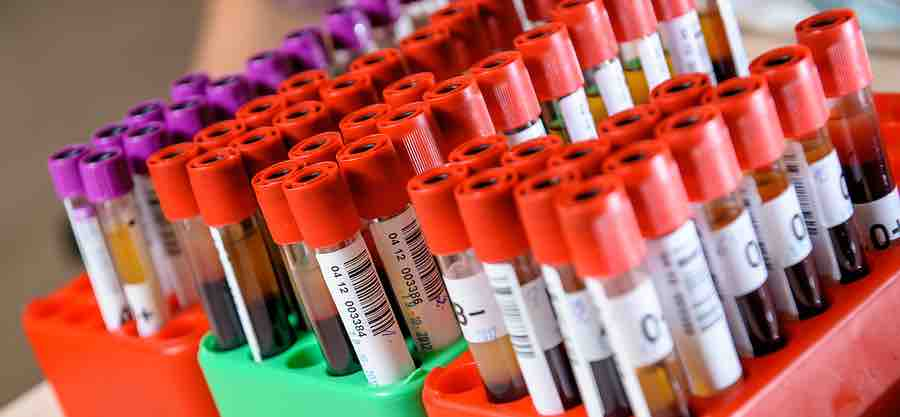
\includegraphics[scale=0.4]{pics/blood-sample}
  \end{center}
  \item 慈善的, 不收費的: pro bono (有別於free! 這個主要指以公共福利為目的)
\end{itemize}

\subsubsection*{需要掌握的句型}
\begin{itemize}
  \itemsep0em
  \item 靠帶來的一點錢過活: live on the money I brought here.
\end{itemize}

\subsection{簽證進度咨詢}
\mybox{\centering \textbf{注意}: 更多筆記被歸納到專題里的``和藍領職業有關的詞", 請參考目錄查找!}
\subsubsection*{需要掌握的單詞短語}
\begin{itemize}
  \itemsep0em
  \item 咨詢: enquire about...
  \item 提交(資料): submit / lodge / \hilight{file}
\end{itemize}

\subsubsection*{需要掌握的句型}
\begin{itemize}
  \itemsep0em
  \item 至今音訊全無: I haven't heard anything since.
  \item 做體檢: \hilight{take} the medical examination / check
  \item 身體好, 硬朗: \hilight{be in good shape / be physically fit}
\end{itemize}

\subsection{車禍賠償}
\mybox{\centering \textbf{注意}: 更多筆記被歸納到專題里的``不同的治療方式", 請參考目錄查找!}
\subsubsection*{需要掌握的單詞短語}
\begin{multicols}{2}
\begin{itemize}
  \itemsep0em
  \item 行車記錄儀: cam recorder
  \item 事務 / 文案律師: solicitor
  \item 巴律師 / 出庭大律師 (戴假髮) / ``大狀": barrister (also known as barrister-at-law)
  \item 人身傷害賠償金: Personal Injury \hilight{Damages}
  \item 激進的(療法): aggressive
  \item 五號公路: \hilight{M5} (M代表motoway)
  \item 丁字路口: T junction
  \item 車牌號: registration number
  \item 路口: intersection / junction / corner
  \item 兩個班次(工作): 2 shifts
  \item 過錯方: party \hilight{at} fault
  \item 判發, 發放: award
\end{itemize}
\end{multicols}

\subsubsection*{需要掌握的句型}
\begin{itemize}
  \itemsep0em
  \item 負責任且有能力的律師: a responsive and \hilight{capable} lawyer.
  \item 撞懵了: I froze (due to the crash).
  \item 腰很痛: sharp pain in my lower back.
  \item 誰有錯: Who was at fault?
  \item 撞向: collide into ...
  \item 直到開庭那天: up to the date of \hilight{hearing}.
  \item 遠遠不夠, 這哪裡夠: be far from enough
\end{itemize}

\subsection{腳踝和膝蓋受傷}
\mybox{\centering \textbf{注意}: 更多筆記被歸納到專題里的``不同的治療方式", 請參考目錄查找!}
\subsubsection*{需要掌握的單詞短語}
\begin{itemize}
  \itemsep0em
  \item 工傷賠償: Worker's Compensation (NAATI可接受簡稱comp, 也有簡稱compo)
  \item 工傷保險: Work Cover
  \item 倉庫: warehouse (主放商品存貨) / depot (t不發音)
  \item 骨科醫生: orthopaedist
  \item 骨外科, \hilight{矯形}外科: orthopaedic surgeon
  \item 狠狠摔: \hilight{nasty} fall
  \item 扭傷 / 拉傷: sprain / strain
  \item 不上班: off-work
  \item \hilight{way} more: ...多了 (相當於much more)
  \item 住房部: Department of Housing
\end{itemize}

\subsubsection*{需要掌握的句型}
\begin{itemize}
  \itemsep0em
  \item 我到單位後不久: Not long after I arrived at my workplace.
  \item 非常想知道: eager to know ...
\end{itemize}

\vspace{15mm}
\begin{center}
  \textbf{************ END OF THE DAY ************}
\end{center}